%   Filename    : chapter_4.tex 
\chapter{Research Methodology}
This chapter discusses the methodology used to develop the text and speech corpus for the Akeanon language. The chapter will be divided into two main parts: Research activities and the calendar of activities for this special problem.

\section{RESEARCH ACTIVITIES}

\begin{figure}[h!]
	\centering
	\caption{Shows the general overview of the methodology for the development of an ASR system for the Akeanon language.}
	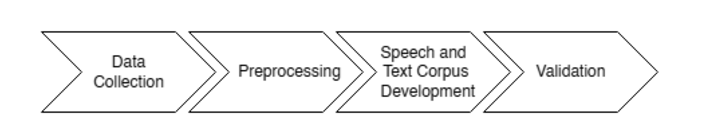
\includegraphics[width=\textwidth]{flowchart.png}
	\label{fig:flowchart}
\end{figure}

\subsection{Data Collection}

\textbf{Collating Pre-existing Online Resources}

For the data collection, the researchers will make use of existing online resources from the website, Bible.com (see Appendix A for permission to use their resources). These resources include recordings and transcriptions of the Akeanon translations of the multiple books and chapters of the Bible.

\textbf{Compiling Akeanon Words and Dictionary Creation}

The researchers will collect equivalent Akeanon words based off on the Swadesh 207 word-list and use the Aklanon to English Dictionary by \citeA{Reyes:1969} as reference. In addition to the Swadesh list, all words from the dictionary made by \shortciteA{Reyes:1969} will be extracted and be converted into text which will later on be included in the lexicon.

\textbf{Phonetic Transcription}

After compiling and converting the Akeanon words extracted from the dictionary into text, their phonetic transcription will also be encoded, using the work of /shortciteA{Rentillo:2022} as reference for Akeanon phonology. Audio transcriptions retrieved from the Bible.com will also have their phonetic transcriptions be encoded.

\textbf{Word Selection for Speech Corpus}

For building the speech corpus, the researchers will prioritize words from the Swadesh list for the voice recordings. Additionally, a selection of 500 random Akeanon words will be prepared for speakers to read.

\textbf{Voice Recording}

A total of 50 native speakers of standard Akeanon will be gathered for the recording of the generated word list. The speakers will be of varying gender and age. For the audio recording, [insert hardware equipment] will be used, having Adobe Audition 2021 as the recording software.

\subsection{Preprocessing}
For preprocessing audio files, Adobe Audition 2021 will be used for recording and audio processing, which will include normalization and noise reduction of the recorded audio.

\subsection{Speech and Text Corpus Development}
The previous steps will set as a precedent for the speech and text corpus development. The development of the text corpus for the Akeanon language involves creating a comprehensive collection of audio transcriptions from pre-existing online resources, dictionary-based word list, and their respective phonetic transcriptions. For the speech corpus, the collated audio transcriptions and word list will be mapped with their corresponding voice recordings and will be annotated accordingly.

\subsection{Validation}
The researchers will collaborate with a linguistic expert, who is also a native speaker of the Akeanon language, in validating the text and speech corpora.

\begin{comment}
This chapter lists and discusses the specific steps and activities that will be performed  to accomplish the project. 
The discussion covers the activities from pre-proposal to Final SP Writing.

\section{Research Activities}
Research activities include inquiry, survey, research, brainstorming, canvassing, consultation, review, interview, observe, experiment, design, test, document, etc.  
Be sure that for each method, process, or algorithm used, there is a justification why that method was chosen.
The methodology also includes the following information:

\begin{itemize}
   \item who is responsible for the task
   \item the resource person to be contacted
   \item what will be done
   \item when and how long will the activity be done
   \item where will it be done
   \item why should be activity be done
\end{itemize}

\textcolor{red}{DO NOT FORGET to cite your references.}

\end{comment}

\section{Calendar of Activities}

% A Gantt chart showing the schedule of the activities should be included as a table. For example:

Table \ref{tab:timetableactivities} shows a Gantt chart of the activities.  Each bullet represents approximately
one week worth of activity.

%
%  the following commands will be used for filling up the bullets in the Gantt chart
%
\newcommand{\weekone}{\textbullet}
\newcommand{\weektwo}{\textbullet \textbullet}
\newcommand{\weekthree}{\textbullet \textbullet \textbullet}
\newcommand{\weekfour}{\textbullet \textbullet \textbullet \textbullet}

%
%  alternative to bullet is a star 
%
\begin{comment}
   \newcommand{\weekone}{$\star$}
   \newcommand{\weektwo}{$\star \star$}
   \newcommand{\weekthree}{$\star \star \star$}
   \newcommand{\weekfour}{$\star \star \star \star$ }
\end{comment}


\begin{table}[ht]   %t means place on top, replace with b if you want to place at the bottom
\centering
\caption{Timetable of Activities} \vspace{0.25em}
\begin{tabular}{|p{2in}|c|c|c|c|c|c|c|c|c|} \hline
\centering Activities (A.Y. 2024-2025) 														& Sep & Oct  & Nov & Dec & Jan & Feb & Mar & Apr & May \\ \hline
Brainstorming and Selection of Topic      													& \weekone & \weektwo &  &  &  &  &  &  & \\ \hline
Drafting and Finalization of Chapter 1 - Introduction 										&  & \weektwo & \weekone &  &  &  &  &  & \\ \hline
Drafting and Finalization of Chapter 2 - Review of Related Literature      					&   &  & \weekthree &  &  &  &  &  &  \\ \hline
Preparation of Letters; UPVREB and Establish Communication for Collaboration     			&   & \weekone &  &  &  &  &  &  &  \\ \hline
Drafting and Finalization of Chapter 3 - Methodologies      								&   &  & \weekone & \weektwo &  &  &  &  &   \\ \hline
Proposal Document Creation in LaTex 														&   &  & \weekone & \weekone &  &  &  &  &  \\ \hline
Proposal Presentation 																		&   &  &  & \weekone &  &  &  &  & \\ \hline
Data Gathering 																				&   &  &  & \weekthree & \weekthree  &  &  &  & \\ \hline
Preprocessing 																				&   &  &  &  &  \weekone  & \weekthree &  &  &  \\ \hline
Drafting and Finalization of Chapter 4 - Results and Discussion 							&   &  &  &  &  & \weekone & \weektwo &  &  \\ \hline
Corpus Development and Validation															&   &  &  &  &  &  & \weekthree & \weekthree &  \\ \hline
Drafting and Finalization of Chapter 5 - Summary and Recommendation							&   &  &  &  &  &  &  & \weektwo & \weektwo \\ \hline
Drafting and Finalization of SP Defense														&   &  &  &  &  &  &  &  & \weekone \\ \hline
SP Defense																					&   &  &  &  &  &  &  &  & \weekone \\ \hline
	
\end{tabular}
\label{tab:timetableactivities}
\end{table}

